\chapter{Realizability}
\label{chap:realizability}

\section{Motivation}
\label{sec:realizability-basic-idea}

Realizability was introduced by Stephen Kleene~\sidecite{KleeneSC:intint} who used it to build a model of intuitionistic arithmetic. We motivate it by asking a practical question: given a mathematical structure (a set equipped with operations and relations satisfying some axioms), what should its implementation look like?

For simple cases, the answer is obvious. A group is implemented by a type whose values represent its elements, a value
representing the neutral element, and functions which compute the group operation and inverses.
But for more interesting structures, especially those arising in mathematical analysis, the answer is less clear. How do we implement the real numbers? Which operations on a compact metric space can be implemented? How do we implement a space of smooth functions? Significant research goes into finding satisfactory answers to such questions~\sidecite{Bla97,Wei00,TZ98,bauer00,bauer10:_canon_effec_subal_class_algeb}.

To explain the basic idea behind realizability we consider a small real-world programming example. Suppose we are asked to design a data structure for the set $\mathsf{Graphs}$ of all finite simple\sidenote{A graph is \defemph{simple} when there is at most one edge between any two vertices.} directed graphs with vertices labeled by distinct integers, such at the graph $G$ shown below:
%
\begin{center}
  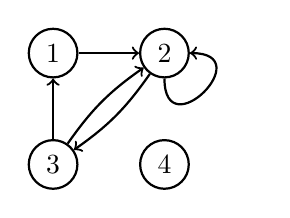
\begin{tikzpicture}
    \node [circle, thick, draw] at ( 45 : 1) (B) {2} ;
    \node [circle, thick, draw] at (135 : 1) (A) {1} ;
    \node [circle, thick, draw] at (225 : 1) (C) {3} ;
    \node [circle, thick, draw] at (315 : 1) (D) {4} ;
    \draw[thick,->] (A) -- (B) ;
    \draw[thick,->] (B) edge [in=0, out=270, looseness=5] (B) ;
    \draw[thick,->] (B) edge [bend left=10] (C) ;
    \draw[thick,->] (C) -- (A) ;
    \draw[thick,->] (C) edge [bend left=10] (B) ;
  \end{tikzpicture}
\end{center}
%
A common representation of graphs uses a pair of lists $(\ell_V, \ell_A)$, where $\ell_V$ is the list of vertex labels and $\ell_A$ the \emph{adjacency list} representing the edges as pairs of labels. For the above graph these would be $\ell_V = [1, 2, 3, 4]$ and $\ell_A = [(1,2), (2,2), (2,3), (3,2), (3,1)]$.
%
Thus we define the datatype of graphs as\sidenote{We use Haskell notation in which $[t]$ is the type of lists of
  elements of type~$t$, and $(t_1, t_2)$ is the cartesian product of types~$t_1$ and~$t_2$.}
%
\begin{lstlisting}[language=Haskell]
type Graph = ([Int], [(Int, Int)])
\end{lstlisting}
%
This is not yet a complete description of the intended representation, as there are representation invariants and conditions not expressed by the type:
%
\begin{itemize}
\item the order in which the vertices and edges are listed is not
  important,
\item every vertex and edge must be listed exactly once, and
\item the source and target of each edge must appear in the list of vertices.
\end{itemize}
%
Such conditions can be expressed in terms of a \defemph{realizability relation}
\begin{equation*}
  r \rz x
\end{equation*}
%
which tells which values~$r$ of the datatype correspond to which elements~$x$ of the set.
%
We read $r \rz x$ as ``$r$ realizes (implements, represents, witnesses) $x$''. In the above example we would write
%
\begin{equation*}
([1, 2, 3, 4], [(1,2), (2,2), (2,3), (3,2), (3,1)]) \rz G,
\end{equation*}
%
and also
%
\begin{equation*}
([3, 2, 1, 4], [(2,2), (1,2), (2,3), (3,2), (3,1)]) \rz G.
\end{equation*}
%
We also want to compute with the elements of $\mathsf{Graphs}$.
%
Programmers intuitively know what this mean, namely to implement, or realize, a map $f : \mathsf{Graphs} \to \mathsf{Graphs}$, is to give a program $p : \mathtt{graph} \to \mathtt{graph}$ which does to realizers what~$f$ does to elements: if $r \rz G$ then $p \, r \rz f(G)$. We say that~$f$ is \defemph{realized} or \defemph{tracked} by~$p$.

\section{Assemblies}
\label{sec:assemblies}

We now give a precise definition of the ideas presented in the previous section.

\begin{definition}
  An \defemph{assembly} over~$(\AA, \subAA)$ a tpca with a sub-tpca is a triple
  $\asm{S} = \xasm{S}$ where $S$ is a set, $|S|$ is a type in~$\AA$, and $\rz_S$ is a relation between $\xAtyp{S}$ and~$S$
  satisfying: for every $x \in S$ there is $\R{x} \in \xAtyp{S}$ such that $\R{x} \rz_S x$.

  An \defemph{assembly map} $f : \asm{S} \to \asm{T}$ between assemblies $\asm{S}$ and $\asm{T}$ is a map $f : S \to T$
  between the underlying sets for which there exists $\R{f} \in \subAtyp{|S| \to |T|}$, called a \defemph{realizer}
  of~$f$, satisfying: if $\R{x} \rz_S x$ then $\defined{\R{f} \, \R{x}}$ and $\R{f} \, \R{x} \rz_T f(x)$.
\end{definition}

We often use the same letter for an element and its realizer, but differentiate between them by using different fonts, for instance the elements $x$, $y$, $f$, $g$ would have realizers $\R{x}$, $\R{y}$, $\R{f}$, $\R{g}$, respectively.

There are many versions of realizability. Ours is known as \defemph{typed relative realizability}. It is \emph{typed}
because we used typed pcas. It is \emph{relative} because maps are realized relative to a choice of a sub-pca. In
typical cases, such as type~2 machines and the graph model from \cref{sec:type-2,sec:graph-model}, $\subAA$ is the
computable part of a topological pca~$\AA$, in accordance with the slogan
%
\begin{center}
  \emph{``Continuous data -- computable functions!''}
\end{center}

When $\subAA = \AA$ we write $\Asm{\AA}$ instead of $\Asm{\AA,\AA}$.

When $\AA$ is untyped the definition of an assembly simplifies a bit because we need mention the (trivial) types.

\begin{definition}
  An \defemph{assembly} over an untyped pca~$\AA$ is a pair $\asm{S} = (S, {\rz_S})$ where $S$ is a set and $\rz_S$ is a relation between~$\AA$ and~$S$, such that for every $x \in S$ there is $r \in A$ and $r \rz_S x$.
\end{definition}

Assemblies and maps over $(\AA, \subAA)$ form a \defemph{category $\AsmA$}.
%
Indeed, if $f : \asm{S} \to \asm{T}$ and $g : \asm{T} \to \asm{U}$ are realized by $\R{f} \in \subAtyp{|S| \to |T|}$
and $\R{g} \in \subAtyp{|T| \to |U|}$, respectively, then their composition $g \circ f$ is realized by
$\tpcalam{x}{|S|}{r\,(q\,x)} = \combS\,(\combK\,r)\,(\combS\,(\combK\,q)\,(\combS\,\combK\,\combK))$.
%
The identity map $\id[S] : \asm{S} \to \asm{S}$ is realized by $\tpcalam{x}{|S|}{x} = \combS\,\combK\,\combK$. 
%
Composition is associative because it is just composition of maps.

\subsection{Modest sets}
\label{sec:modest-sets}

In the definition of assemblies, nothing prevents several elements from sharing a common realizer. We sometimes want
to prohibit such anomalies.

\begin{definition}
  An \defemph{modest} assembly $\asm{S}$, also called a \defemph{modest set},\sidenote{The terminology was suggested by Dana Scott. It refers to the fact that the cardinality of a modest set~$\asm{S}$ does not exceed the cardinality of $\xAtyp{S}$.} is an assembly in which elements do not share realizers:
  %
  \begin{equation*}
    \all{r}{\xAtyp{S}}{
      \all{x,y \in S}
      (r \rz_S x \land r \rz_S y \implies x = y)
    }.
  \end{equation*}
  %
  We let $\ModA$ be the full subcategory of $\AsmA$ on the modest sets.
\end{definition}

Most structures in computable mathematics turn out to be modest, but assemblies are needed also, and they form a richer category than the modest sets.

\subsection{First examples of assemblies}
\label{sec:examples-assemblies}

To gain a bit of intuition about assemblies, we look at several concrete examples. Unless stated otherise, we assume that all assemblies are constructed over a chosen pca with sub-pca $(\AA, \subAA)$.

\subsubsection{The unit assembly}
\label{sec:asm-unit}

Let $\unit$ be a type such that $\subAtyp{\unit}$ is inhabited.
It always exists, because there is at least one type $s$, and then
$\Atyp{s \to s \to s}$ contains $\combK_{s,s}$.
%
The \defemph{terminal assembly} $\one = (\set{\star}, \unit, {\rz_\one})$ has the trivial realizability relation, $r \rz_\one \star$ for all $r \in \subAtyp{t}$.

\begin{exercise}
  Show that $\one$ is the terminal object\sidenote{An object $T$ in a category is \defemph{terminal} when there is precisely one morphism to $T$ from every object.}
  in $\AsmA$. Conclude from this that a different choice of $\unit$ results in an isomorphic copy of~$\one$.
\end{exercise}

The morphisms $\one \to \asm{S}$ corresponds to those elements of~$S$ that are realized by elements of $\subAtyp{|S|}$. Indeed, if $f : \star \to S$ is realized by $\R{f} \in \subAtyp{\unit \to |S|}$ then $f \, \star$ is realized by $\R{f} \, t \in \subAtyp{|S|}$, for any $t \in \subAtyp{\unit}$. Conversely, if $a \in S$ is realized by $\R{a} \in \subAtyp{|S|}$ then $\star \mapsto a$ is $\tpcalam{x}{\unit}{\R{a}}$.

This may be a good moment to point out the difference between the \defemph{global points} of~$\asm{S}$, which is the set of morphisms $\one \to \asm{S}$, and the \defemph{underlying set~$S$} of~$\asm{S}$. Both induce functors $\AsmA \to \Set$, which need not be equivalent, unless $\AA = \subAA$.


\subsubsection{Natural numbers}
\label{sec:asm-natural-numbers}

Suppose $(\AA, \subAA)$ is an n-tpca. Let $\asm{N} = (\NN, \ttnat, {\rz_N})$ be the set of natural numbers~$\NN$ realized by the numerals, for all $r \in \Atyp{\ttnat}$ and $n \in \NN$,
%
\begin{equation*}
  r \rz_N n \iff
  r = \overline{n}.
\end{equation*}
%
The successor $n \mapsto n + 1$ is realized by~$\combSucc$, and $0 \in \mathbb{N}$ is a global point because $\numeral{0} \in \subAtyp{\ttnat}$.

The assembly $\mathbb{N}$ is the natural numbers object. Indeed, given an assembly $\asm{S}$ with $z \in \asm{S}$ realized by $\mathtt{z} \in \subAtyp{|S|}$, and $f : \asm{S} \to \asm{S}$, the unique map $\overline{f} : \asm{N} \to \asm{S}$ satisfying, for all $n \in \NN$,
%
\begin{equation*}
  \overline{f} \, 0 = 0
  \qquad\text{and}\qquad
  \overline{f} \, (n + 1) = f (\overline{f} n)
\end{equation*}
%
is realized by $\combRec \, \mathtt{z} \, \mathtt{f}$.


\subsubsection{Boolean, semidecidable, and classical truth values}
\label{sec:asm-two-element}

Let us work in the category $\Asm{\klone}$ over Kleene's first algebra and look at assembly structures on the set $2 = \set{0, 1}$.

First, we have the trivial structure, namely the assembly of \defemph{classical truth values} $\nabla 2 = (2, {\rz_{\nabla 2}})$ -- the notation will become clear in \cref{sec:nabla}, and the nomenclature a bit later -- with the trivial realizability relation $n \rz_{\nabla \two} b$ for all $k \in \NN$ and $b \in 2$.

Second, we have the assembly of \defemph{Boolean values} $\two = (2, {\rz_{2}})$ where $n \rz_2 b$ if, and only if $n = b$.

The assemblies $\nabla 2$ and $\two$ are \emph{not} isomorphic because every assembly map $\nabla 2 \to \two$ is constant, although the identity map is an assembly map $\two \to \nabla 2$.

There are still more two-element assemblies, for instance the assembly of \defemph{semidecidable values} $\asm{S} = (2, {\rz_S})$ given by
%
\begin{equation*}
  n \rz b \iff
  (\divergent{\pr{n}{n}} \land b = 0) \lor (\defined{\pr{n}{n}} \land b = 1).
\end{equation*}
%
Again, the identity map is realized as an assembly map $\two \to \asm{S}$, but not the other way around.

\begin{exercise}
  Why is identity not realized as a map $\asm{S} \to \two$?
\end{exercise}


\subsubsection{Real numbers}
\label{sec:asm-real-numbers}

As our third example we ask how to equip the real numbers with a realizability structure. Here we give the correct answer, but leave it unexplained for the time being.

We work with an nr-tpca $\AA$ with a sub-n-tpca $\subAA$. Intuitively speaking, a realizer for $x \in \RR$ should allow us to compute arbitrarily good approximations of~$x$, so we define the relation $\rz_R$ between $\Atyp{\ttnat \to \ttnat \times \ttnat \times \ttnat}$ by stipulating that $\R{x} \rz_R x$ holds if, and only if,
%
\begin{equation*}
  \all{k \in \NN} \some{a, b, c \in \NN}
  \R{x} \, \overline{k} = (\overline{a}, \overline{b}, \overline{c})
  \land |x - \frac{a - b}{1 + b}| < 2^{-k}.
\end{equation*}
%
The triple of numbers $(a, b, c)$ is just a clumsy way of encoding the rational $\frac{a - b}{c}$, so in essence $\R{x}$ computes a sequence of rationals such that the $k$-th term is within~$2^{-k}$ of~$x$.

The assembly of real numbers $\asm{R} = (R, \ttnat \to \ttnat \times \ttnat \times \ttnat, {\rz_R})$ has as its underlying set the realized reals
%
\begin{equation*}
  R = \set{x \in \RR \such \some{\R{x} \in \Atyp{\ttnat \to \ttnat \times \ttnat \times \ttnat}} \R{x} \rz_R x}.
\end{equation*}
%
Which reals are so realized depends on the choice of~$\AA$. For example, first Kleene algebra realizes the \defemph{Turing computable reals}, whereas the second Kleene algebra realizes all reals.

\subsection{The constant assemblies}
\label{sec:nabla}

The extreme case of elements sharing the same realizer happens when
all elements of a set share all realizers. Assemblies with this
property are called the \defemph{constant assemblies}.

Let $t$ be a type such that $\subAtyp{t}$ is inhabited. Such a type
always exists, because there is at least one type $s$, and then
$\Atyp{s \to s \to s}$ contains $\combK_{s,s}$. Given any set $X$, let
%
\begin{equation*}
  \nabla X = (X, t, {\rz_{\nabla X}})
\end{equation*}
%
be the assembly whose underlying set is~$X$ and the realizability relation is trivial, i.e., $r \rz_{\nabla X} x$ for all $x \in X$ and $r \in A_t$.

If $f : X \to Y$ is any map between sets~$X$ and~$Y$ then~$f$ is a morphism $\nabla f : \nabla X \to \nabla Y$ because it is tracked by $\tpcalam{x}{t}{x}$. Thus~$\nabla$ is a functor
%
\begin{equation*}
  \nabla : \Set \to \AsmA.
\end{equation*}
%
Up to natural isomorphism, $\nabla$ is independent of the choice of
type~$t$. We will study the properties of $\nabla$ later on. For now
we notice that $\nabla$ is full and faithful, which means that
$\AsmA$ contains the category of sets as a full
subcategory.

The functor $\nabla$ is devoid of any computational content because it
represents a set~$X$ by a trivial realizability relation which conveys
no information at all about the elements of~$X$. Consequently, from
the realizers we cannot compute anything interesting regarding~$X$.

\begin{exercise}
  Let $\Gamma : \AsmA \to \Set$ be the forgetful functor which assigns to an assembly its underlying set, and to an
  aseembly map the underlying set-theoretic function. Show that~$\Gamma$ is left adjoint to~$\Delta$.
\end{exercise}

\section{Equivalent formulations}
\label{sec:equivalent-formulations}

Assemblies and modest sets have several equivalent formulations, which were formulated by different communities for particular choices of $(\AA, \subAA)$, each using their own notation and terminology. In this section we review the equivalent formulations, and in \cref{sec:schools} show how various ``schools of computable mathematics'' arise as special instances.

\subsection{Existence predicates}
\label{sec:existence-predicates}

A realizability relation $\rz_S$ is a subset of $\xAtyp{S} \times S$. By transposition it may be equivalently expressed
as a map $\Ex_S : S \to \pow{\xAtyp{S}}$. The correspondence is
%
\begin{equation*}
  \R{x} \rz_S x \iff \R{x} \in \Ex_S(x).
\end{equation*}
%
Because every $x$ is realized by something, $\Ex_S(x)$ always contains at least one element. Thus an assembly $\xasm{S}$ may be equivalently presented as a triple $(S, |S|, \Ex_S)$ where $\Ex_S : S \to \pow{\xAtyp{S}}$ is a map, called the \defemph{existence predicate}, such that $\Ex_S(x)$ contains at least one element for every $x \in S$. The name suggests that the elements of $\Ex_S(x)$ are computational witnesses for ``existence of~$x$''.

An assembly $S$ is modest if, and only if, $\Ex_S(x) \cap \Ex_S(y) \neq \emptyset$ implies $x = y$.

Under this formulation a map $f : \asm{S} \to \asm{T}$ is realized if there exists $\R{f} \in \subAtyp{|S| \to |T|}$ such that, for all $x \in S$ and $\R{x} \in \Ex_S(x)$, $\defined{\R{f}\,\R{x}}$ and $\R{f}\,\R{x} \in \Ex_T(f(x))$.

\subsection{Representations}
\label{sec:representations}

By transposing $\rz_S$ the other way around we obtain \defemph{representations}. Suppose first that $S$ is a modest set. Since every realizer $r \in \xAtyp{S}$ realizes at most one $x \in S$, we may define a partial map $\delta_S : \xAtyp{S} \parto S$ by
%
\begin{equation*}
  \delta_S(r) = x \iff r \rz_S x.
\end{equation*}
%
The map $\delta_S$ is surjective because every $x \in S$ is realized, but it need not be defined everywhere. The triple $(S, |S|, \delta_S)$ uniquely describes the modest set~$S$. The map $\delta_S$ is called a \defemph{representation} of~$S$.

A map $f : S \to T$ is realized or tracked by $\R{f} \in \subAtyp{|S| \to |T|}$ when, for all $\R{x} \in \dom{\delta_S}$, $\defined{\R{f}\,\R{x}}$ and $\delta_T(\R{f}\,\R{x}) = f(\delta_S(x))$.

Representations and realized maps form a category~$\Rep{\AA,\subAA}$, which is equivalent to $\Mod{\AA, \subAA}$.

When we transpose $\rz_S$ for a a general assembly $\asm{S}$ the result is a \defemph{multi-valued representation}, which is a map $\delta_S : \xAtyp{S} \multito \pow{S}$ that takes each $r \in \xAtyp{S}$ to the (possibly empty) set of elements it realizes,
%
\begin{equation*}
  \delta_S(r) = \set{ x \in S \such r \rz_S x}.
\end{equation*}
%
The map is surjective in the sense that for every $x \in S$ there is $r \in \xAtyp{S}$ such that $x \in \delta_S(r)$.

To summarize, there are three ways of specifying the realizability structure of an assembly: with a realizability relation $\rz_S$, an existence predicate~$\Ex_s$, and a multi-valued representation $\delta_S$. Each determines the other two by
%
\begin{equation*}
  r \rz_S x \iff
  r \in \Ex_S(x) \iff
  x \in \delta_S(r).
\end{equation*}


\subsection{Partial equivalence relations}
\label{sec:pers}

This formulation only works for modest sets. With each modest set~$S$ we may associate a partial equivalence relation\sidenote{A \defemph{partial equivalence relation} is a transitive symmetric relation.} (per) $\per_S$ on $\xAtyp{S}$ which relates~$q$ and~$r$ when they realize the same element:
%
\begin{equation*}
  q \per_S r \iff
  \some{x \in S} q \rz_S x \land r \rz_S x.
\end{equation*}
%
The pair $(|S|, {\per_S})$ suffices for the reconstruction of the
original modest set, up to isomorphism, which we show next.

Let $(\AA, \subAA)$ be a tpca with a sub-tpca. A \defemph{partial
  equivalence relation} on~$\AA$ is a pair $S = (|S|, {\per_S})$ where
$|S|$ is a type and $\per_S$ is a transitive and symmetric
relation on $\xAtyp{S}$. A realizer $r \in \xAtyp{S}$ is \defemph{total} if
$r \per_S r$. The set of total realizers is denoted by $\|S\| = \set{r
  \in \xAtyp{S} \such r \per_S r}$. Each $r \in \|S\|$ determines
the equivalence class $[r]_S = \set{q \in \xAtyp{S} \such r \per_S q}$.

An \defemph{extensional realizer} between pers $S$ and $T$ is $p \in
\subAtyp{|S| \to |T|}$ such that, for all $q, r \in \xAtyp{S}$, if $q
\per_S r$ then $\defined{p\,q}$, $\defined{p\,r}$, and $p\,q \per_T
p\,r$. Extensional realizers $p$ and $p'$ are \defemph{equivalent} when
$q \per_S r$ implies $p\,q \per_T p'\,r$.

Pers and equivalence classes of extensional realizers form a category
$\Per{\AA, \subAA}$ whose objects are pers on~$\AA$ and morphisms are
equivalence classes of extensional realizers. The composition of $[p]
: S \to T$ and $[q] : T \to U$ is $[q \circ p] : S \to U$ where $q
\circ p = \tpcalam{x}{|S|}{q\,(p\,x)}$. The identity morphism
$\id[S] : S \to S$ is represented by $\tpcalam{x}{|S|} x$. It
is easy to check that this forms a category.

Let $S$ and $T$ be pers over $(\AA, \subAA)$. A morphism between them
may be alternatively described as a function $f : \|S\|/{\per_S} \to
\|T\|/{\per_T}$ between the equivalence classes for which there exists
a realizer $p \in \subAtyp{|S| \to |T|}$ that tracks it: for every
equivalence class $[r]_S$, $\defined{p\,r}$ and $[p\,r]_T = f([r]_S)$.

\begin{lemma}
  \label{lemma:iso-assembly}
  %
  Suppose $\asm{S}$ is an assembly, $T$ is a set, and $f : T \to S$ is
  a bijection. Then $\asm{S}$ is isomorphic to $\asm{T} = (T, |S|,
  {\rz_T})$ where $r \rz_T x$ is defined as $r \rz_S f(x)$.
\end{lemma}


\begin{proof}
  The map $f$ is a morphism from $\asm{S}$ to $\asm{T}$ because it is
  tracked by~$\tpcalam{x}{|S|}{x}$. Similarly, $\inv{f}$ is a
  morphism because it is also tracked by the same realizer. Obviously,
  $f$ and $\inv{f}$ are inverses of each other.
\end{proof}


\begin{proposition}
  The categories $\Mod{\AA, \subAA}$ and $\Per{\AA, \subAA}$ are
  equivalent.
\end{proposition}

\begin{proof}
  A modest set $\xasm{S}$ determines a per $(S, {\per_S})$,
  as described above. A morphism $f : S \to T$ which is tracked by $p
  \in \subAtyp{|S| \to |T|}$ determines a morphism of pers $[p] : (S,
  {\per_S}) \to (T, {\per_T})$. This defines a functor $F : \Mod{\AA,
    \subAA} \to \Per{\AA, \subAA}$.

  In the other direction the functor $G : \Per{\AA, \subAA} \to
  \Mod{\AA, \subAA}$ sends a per $(|T|, {\per_T})$ to the modest set
  $(\|T\|/{\per_T}, |T|, {\rz_T})$ whose realizability relation is
  %
  \begin{equation*}
    r \rz_T [q] \iff r \per_T q.
  \end{equation*}
  %
  A morphism $[p] : (S, {\per_S}) \to (T, {\per_T})$ is mapped to the
  map $G [p] : \|S\|/{\per_S} \to \|T\|/{\per_T}$, defined by $G [p]
  [r]_S = [p\,r]_T$, which is obviously tracked by~$p$.

  The functors $F$ and $G$ form an equivalence of categories. The
  composition $F \circ G$ is actually equal to identity, as is easily
  verified. A modest set~$\xasm{S}$ is isomorphic to
  $G(F(S))$ by \cref{lemma:iso-assembly} applied to the bijection
  which takes an $x \in S$ to $[r]_{G(F(S))}$, where $r \in \xAtyp{S}$
  is any realizer such that $r \rz_S x$. We leave the verification
  that the isomorphisms are natural as exercise.
\end{proof}


\subsection{Equivalence relations}
\label{sec:ers}

A per $(|S|, {\per_S})$ may be viewed as an equivalence relation on
$\|S\| = \set{r \in \xAtyp{S} \such r \per_S r}$. This gives us yet
another equivalent formulation of modest sets, this time in terms of
equivalence relations.

The category $\Er{\AA, \subAA}$ of equivalence relations has as objects triples $(S, |S|, {\equiv_S})$ where $|S|$ is a
type, $S \subseteq \xAtyp{S}$, and $\equiv_S$ is an equivalence relation on~$S$. As in the case of pers, a morphism
$(S, |S|, {\equiv_S}) \to (T, |T|, {\equiv_T})$ is represented by an extensional realizer
$p \in \subAtyp{|S| \to |T|}$.

The difference between pers and equivalence relations is mostly a
bureaucratic one. Nevertheless, it is useful to know about $\Er{\AA,
  \subAA}$ because sometimes we can describe it in enlightening
alternative ways, e.g., in \cref{sec:equilogical-spaces} we
describe pers on the graph model as equivalence relations on
topological spaces.

\section{Applicative functors}
\label{sec:applicative-functors}


\index{functor!induced by applicative morphism}%
\index{applicative!morphism!functor induced by}%

Categories of assemblies themselves form a category whose morphisms are functors induced by simulations, known as \emph{applicative functors}. These were defined and studied by John Longley~\cite{Longley:94}, and are the appropriate notion of morphisms of assemblies, as well as realizability toposes. We review their definition and several basic results about them, which we cannot do without assuming some knowledge of basic category theory.

A simulation $\rho: (\EE, \subEE) \pcato (\FF, \subFF)$ induces an \defemph{applicative functor}
%
\begin{equation*}
  \ff{\rho}: \Asm{\EE, \subEE} \longrightarrow \Asm{\FF, \subFF}
\end{equation*}
%
which maps an assembly $\asm{S} = \xasm{S}$ over $(\EE, \subEE)$ to the assembly
$\ff{\rho} \, \asm{S}$ over $(\FF, \subFF)$, whose underlying set is $S$ and
%
\begin{align*}
  |\ff{\rho} \asm{S}| &= |S|,
  &
  q \rz_{\ff{\rho} \asm{S}} x
  \iff \some{r \in \EE} q \in \rho[r] \land r \rz_S x.
\end{align*}
%
That is, $\ff{\rho}$ replaces realizers in~$\EE$ with their simulations in~$\FF$.

Suppose $r \in \subFF$ is a realizer for~$\rho$. An assembly map $f: \asm{S} \to \asm{T}$, realized by $\mathtt{f} \in \typ{\EE}{|S| \to |T|}$, is mapped by $\ff{\rho}$ to the same underlying map $\ff{\rho}\,f = f$, which is realized by $r \, \mathtt{g}$ for any $\mathtt{g} \in \rho[\mathtt{f}]$.

\begin{exercise}
  Prove that and applicative functor induced by a \emph{discrete} simulation restricts to modest sets.
\end{exercise}

The properties of the induced applicative functor depend on the properties of the simulation, as follows. (We presume existence of categorical structure on assemblies which will only be established in \cref{cha:categ-structure}.)

\begin{proposition}
  \label{th:applicative_functor_properties}%
  %
  Let $\rho: (\EE, \subEE) \pcato (\FF, \subFF)$ be a simulation.
  % 
  \begin{enumerate}
  \item
    %
    The functor $\ff{\rho}$ is faithful  and it preserves finite limits.
  \item
    %
    If $\rho$ is projective then $\ff{\rho}$ preserves projective objects.
  \item
    %
    If $\rho$ is decidable then $\ff{\rho}$ preserves finite colimits and the natural numbers object.
  \end{enumerate}
\end{proposition}

\begin{proof}
  The functor $\ff{\gamma}$ preserves finite limits
  by~\cite[Proposition~2.2.2]{Longley:94}. It is faithful
  because it acts trivially on morphisms.
  %
  For the second claim see~\cite[Theorem~2.4.12]{Longley:94}, and for the third one~\cite[Theorem~2.4.19]{Longley:94}.
\end{proof}

Adjunctions and equivalences between simulations carry over to the induced morphisms.

\begin{theorem}
  \label{th:applicative_adjunction_functor_adjunction}%
  Consider simulations
                                %
  \begin{align*}
    \delta &: (\EE, \subEE) \pcato (\FF, \subFF),
    &
    \gamma &: (\FF, \subFF) \pcato (\EE, \subEE).
  \end{align*}
                                %
  \begin{enumerate}
  \item If $\gamma \dashv \delta$ is an adjoint pair, then
    $\ff{\gamma} \dashv \ff{\delta}$ is an adjunction of functors.
    %
    \index{adjunction!induced by simulation adjunction}%
    %
  \item If $\gamma \dashv \delta$ is an adjoint inclusion then the counit of the adjunction $\ff{\gamma} \dashv \ff{\delta}$ is a natural isomorphism.
    %
  \item If $\gamma \dashv \delta$ is an adjoint retraction then the unit of the adjunction $\ff{\gamma} \dashv \ff{\delta}$ is a natural isomorphism.
  \item If $\gamma$ and $\delta$ form an equivalence, then so do $\ff{\gamma}$ and
    $\ff{\delta}$.
  \end{enumerate}
\end{theorem}

\begin{proof}
  The first three claims are subsumed by the easy part of~\cite[Proposition 2.5.9]{Longley:94}, except that we are using simulations on pcas with sub-pcas. Also, we are restricting attention to categories of assemblies rather than realizability toposes, but this is not a problem because by applicative functors on realizability toposes restrict to assemblies.

  That equivalences of simulations induce equivalences of categories is shown in~\cite[Theorem 2.5.6]{Longley:94}.
\end{proof}

The construction of assemblies and induced applicative functors extends to a 2-functor between 2-categories. Indeed, given $\gamma, \delta : (\EE, \subEE) \pcato (\FF, \subFF)$ such that $\gamma \preceq \delta$, there is an induced natural transformation $\zeta : \ff{\gamma} \natto \ff{\delta}$ defined by
%
\begin{equation*}
  \zeta_{\asm{S}} = \id[S] : \ff{\gamma}\,\asm{S} \to \ff{\delta}\,\asm{S}.
\end{equation*}
%
This is a valid definition, for if $t \in \subFF$ is a translation witnessing $\gamma \preceq \delta$, then $t$ tracks every $\zeta_{\asm{S}}$, and the naturality condition is trivial.

An applicative functor induced by $\rho : (\EE, \subEE) \pcato (\FF, \subFF)$ commutes up to natural isomorphism with the constant assembly functor~$\nabla$ from \cref{sec:nabla},
%
\begin{equation*}
  \xymatrix{
    {\Asm{\EE, \subEE}}
    \ar[rr]^{\ff{\rho}}
    & &
    {\Asm{\FF, \subFF}}
    \\
    & {\Set}
    \ar[ur]_{\nabla}
    \ar[ul]^{\nabla}
  }
\end{equation*}
%
as well as with the underlying set functor~$\Gamma$,
%
\begin{equation*}
  \xymatrix{
    {\Asm{\EE, \subEE}}
    \ar[rr]^{\ff{\rho}}
    \ar[dr]_{\Gamma}
    & &
    {\Asm{\FF, \subFF}}
    \ar[dl]^{\Gamma}
    \\
    & {\Set}
  }
\end{equation*}
%
See \cite[Proposition 2.2.4]{Longley:94} for the proof.

%%% Local Variables: 
%%% mode: latex
%%% TeX-master: "notes-on-realizability"
%%% End: 
